\documentclass[12pt,a4paper]{article}

\usepackage[utf8]{inputenc}
\usepackage[T1]{fontenc}
\usepackage[portuguese]{babel}
\usepackage{graphicx}
\usepackage{geometry}
\usepackage{hyperref}
\usepackage{float}
\usepackage{amsmath}
\usepackage{booktabs}
\usepackage{listings}
\usepackage{xcolor}
\usepackage{setspace}

\geometry{a4paper, margin=2.5cm}
\setstretch{1.5} % Espaçamento de 1.5 para formato acadêmico

\definecolor{codegreen}{rgb}{0,0.6,0}
\definecolor{codegray}{rgb}{0.5,0.5,0.5}
\definecolor{codepurple}{rgb}{0.58,0,0.82}
\definecolor{backcolour}{rgb}{0.95,0.95,0.92}

\lstdefinestyle{mystyle}{
    backgroundcolor=\color{backcolour},   
    commentstyle=\color{codegreen},
    keywordstyle=\color{magenta},
    numberstyle=\tiny\color{codegray},
    stringstyle=\color{codepurple},
    basicstyle=\ttfamily\footnotesize,
    breakatwhitespace=false,         
    breaklines=true,                 
    captionpos=b,                    
    keepspaces=true,                 
    numbers=left,                    
    numbersep=5pt,                  
    showspaces=false,                
    showstringspaces=false,
    showtabs=false,                  
    tabsize=2
}
\lstset{style=mystyle}

\title{\textbf{Modelagem, Implementação e Análise Comparativa de Estruturas em Árvore Especializadas}}
\author{
    \textbf{Arthur de Oliveira Mendonça} \\
    Engenharia da Computação \\
    Centro Federal de Educação Tecnológica de Minas Gerais (CEFET-MG) - Campus Divinópolis \\
    Disciplina: Algoritmos e Estruturas de Dados II \\
    Professor: Michel Pires da Silva
}
\date{Setembro de 2026}

\begin{document}

\maketitle

\begin{abstract}
Este artigo documenta o projeto prático focado na implementação e avaliação de cinco estruturas de dados arbóreas avançadas: Splay Tree, Treap, Trie, Patricia Tree e KD-Tree. As estruturas foram desenvolvidas em Dart, visando uma arquitetura modular capaz de se conectar a um front-end nativo em Flutter, viabilizando o rastreamento visual passo-a-passo. Realizaram-se extensos experimentos de \textit{benchmarking} para avaliar o tempo de execução (inserção e busca) e o consumo de memória frente a diferentes distribuições de dados (aleatórios, ordenados e enviesados). Os resultados comprovam características assintóticas teóricas, como a degeneração computacional em casos não-aleatórios, além de destacar a Patricia Tree no papel de economia espacial em relação a dicionários.
\end{abstract}

\newpage
\section{Introdução}
O armazenamento, recuperação e manipulação eficiente de grandes volumes de dados são pilares da Engenharia da Computação moderna. O estudo de Estruturas de Dados clássicas, como as Árvores Binárias de Busca (BST) e Árvores AVL, oferece uma base teórica robusta. No entanto, demandas específicas — como localidade de acesso, consultas parciais em strings (prefixos) e cálculos de distância espacial — tornam o uso de implementações padronizadas uma escolha ineficiente.

Este trabalho aborda o desenvolvimento teórico e prático de cinco tipos de árvores voltadas para domínios altamente especializados:
\begin{enumerate}
    \item \textbf{Splay Tree:} Auto-ajustável para otimização de localidade temporal de referência.
    \item \textbf{Treap:} Árvore cartesiana randomizada, dispensando regras complexas de rotações.
    \item \textbf{Trie (Árvore de Prefixos):} Mapeamento posicional para recuperação de conjuntos de caracteres.
    \item \textbf{Patricia Tree:} Variação otimizada da Trie para compressão de caminhos únicos, minimizando \textit{overhead} de memória.
    \item \textbf{KD-Tree:} Particionamento multidimensional do espaço, implementada aqui em bidimensionalidade ($K=2$).
\end{enumerate}

Para alcançar a compreensão integral dessas estruturas, a proposta vai além do algorítmico, implementando um aplicativo móvel no \textit{framework} Flutter que executa a captura do estado interno das árvores a cada instrução (Arquitetura de \textit{Snapshots}), desenhando topologias dinâmicas na interface visual do usuário.

\section{Fundamentação Teórica e Modelagem}

\subsection{Splay Tree (Árvore de Espalhamento)}
A Splay Tree, desenvolvida por Sleator e Tarjan (1985), abandona as propriedades de balanceamento estrito de altura. Seu motor principal é a heurística de \textit{Splaying}, garantindo que a chave recém-acessada ou inserida chegue à raiz através de cascatas de rotações. Estas operam em três fluxos primordiais:
\begin{itemize}
    \item \textbf{Zig:} Apenas o pai existe (rotação simples à raiz).
    \item \textbf{Zig-Zig:} A chave e seu pai estão na mesma direção (ex: ambos são filhos esquerdos). A rotação ocorre no avô e depois no pai.
    \item \textbf{Zig-Zag:} Posições alternadas (esquerda-direita). Uma rotação tradicional dupla de AVL.
\end{itemize}
Esta mecânica fornece um tempo amortizado de $\mathcal{O}(\log N)$, tornando a Splay Tree excepcional para rotinas de \textit{cache}, onde $20\%$ dos dados são acessados $80\%$ das vezes.

\subsection{Treap}
A Treap (\textit{Tree + Heap}) une as propriedades matemáticas das Árvores Binárias de Busca às propriedades de Max-Heap (ou Min-Heap). A ideia seminal, proeminente na computação probabilística, associa cada nova chave a uma \textit{prioridade aleatória}.

Pela regra da BST: Se $v$ pertence à subárvore esquerda de $u$, então $v.chave < u.chave$. Pela regra do Heap: A prioridade do nó pai deve ser estritamente maior (ou menor) do que a prioridade de seus filhos, ou seja, $u.prioridade > v.prioridade$.

O balanceamento surge da probabilidade. Considerando números aleatórios contínuos distribuídos uniformemente, as rotações tendem inevitavelmente a equilibrar os nós nas subárvores.

\subsection{Trie}
A estrutura da Trie afasta-se de nós que carregam dados escalares para focar em arrays ou dicionários (HashMaps) mapeando o alfabeto. Ao invés da busca depender da quantidade de registros inseridos ($N$), a complexidade desce para o comprimento da chave buscada ($M$). 

O desafio da Trie convencional é a ocupação da memória. Para inserir uma string única de tamanho 20, 20 novos nós completos precisam ser alocados no sistema (podendo possuir instâncias inteiras do alfabeto não utilizadas), resultando em alta dispersão espacial de memória.

\subsection{Patricia Tree (Radix Compacta)}
A \textit{Practical Algorithm to Retrieve Information Coded in Alphanumeric} (PATRICIA), ou Radix Tree Compacta, resolve o calcanhar de Aquiles da Trie condensando o grafo. Se um nó só possui uma única bifurcação no seu percurso, seu caractere e os de seus descendentes lineares diretos são concatenados em uma única \textit{label}. 

\subsection{KD-Tree}
Base para computação gráfica e GIS (\textit{Geographic Information System}), a KD-Tree estende os paradigmas comparativos para além de uma dimensão. Ao inserir um nó de coordenadas bidimensionais $(x, y)$, a KD-Tree checa a paridade da profundidade. Em níveis pares (0, 2, 4...) compara-se a coordenada horizontal $x$. Em níveis ímpares (1, 3, 5...), compara-se a vertical $y$. Isso divide recursivamente o plano em retângulos cada vez menores, acelerando brutalmente consultas de vizinhança na geometria.

\section{Detalhes de Implementação e Arquitetura}
Toda a lógica de Domínio (Business Logic) e de interface gráfica foi construída através do ecossistema Google (Dart e Flutter), provendo um código estritamente orientado a objetos, tipado estaticamente, e capaz de transposição para ecossistemas Web, iOS, e Android simultaneamente.

\subsection{Sistema de Snapshots}
Para cumprir a exigência da demonstração interativa passo a passo das operações, desenvolveu-se a classe \texttt{TreeSnapshot}. Durante todas as operações modificadoras de estado (Insert, Delete), uma transcrição visual (`toMap()`) da árvore é instanciada e alocada na memória de histórico da respectiva classe de domínio.

\begin{lstlisting}[language=Java, caption=Captura do Estado em Snapshot nas operações]
void _recordHistory(String operation, T key) {
    history.add(TreeSnapshot(
      step: history.length + 1,
      operation: operation,
      key: key,
      rootKey: root?.key,
      treeMap: root?.toMap(),
      inorder: inorder(), // Armazena a listagem em-ordem dinâmica
    ));
}
\end{lstlisting}

Os Snapshots alimentam o Canvas renderizado pela classe \texttt{TreePainter} que lê de forma recursiva os campos de dicionários `left` e `right` instanciando primitivas visuais.

\section{Análise Teórica de Complexidade}
Abaixo encontra-se a modelagem teórica computacional das estruturas analisadas:

\begin{table}[H]
\centering
\begin{tabular}{@{}lccc@{}}
\toprule
\textbf{Estrutura} & \textbf{Inserção} & \textbf{Busca} & \textbf{Espaço (Pico)} \\ \midrule
Splay Tree & $\mathcal{O}(\log N)$* & $\mathcal{O}(\log N)$* & $\mathcal{O}(N)$ \\
Treap & $\mathcal{O}(\log N)$** & $\mathcal{O}(\log N)$** & $\mathcal{O}(N)$ \\
Trie & $\mathcal{O}(M)$ & $\mathcal{O}(M)$ & $\mathcal{O}(N \times M)$ \\
Patricia Tree & $\mathcal{O}(M)$ & $\mathcal{O}(M)$ & $\mathcal{O}(N)$ \\
KD-Tree (2D) & $\mathcal{O}(N)$*** & $\mathcal{O}(N)$*** & $\mathcal{O}(N)$ \\ \bottomrule
\end{tabular}
\caption{Quadro Teórico: (*) Amortizado; (**) Caso Médio (Alta prob.); (***) Em dados sequencialmente ordenados que forçam linhas retas na geometria do plano.}
\end{table}

\section{Experimentos e Resultados Práticos}
Foi idealizado um sistema de Benchmarking que injeta cargas variáveis nas árvores. Foram gerados dados perfeitamente ordenados (Pior caso de árvores sem balanceamento, \textit{Sorted}), completamente pseudo-aleatórios (\textit{Random}) e enviesados (\textit{Skewed}, para analisar efeito cache). Os testes simularam a inserção de até dezenas de milhares de elementos sequenciais. 

\subsection{Comportamento do Tempo de Inserção}
A Figura \ref{fig:insert} corrobora o comportamento fundamental logarítmico para as árvores binárias convencionais (Splay, Treap) quando nutridas com dados caóticos. A Treap apresenta leve superioridade nominal devido à ausência de recálculos de balanceamento complexos na base.

\begin{figure}[H]
    \centering
    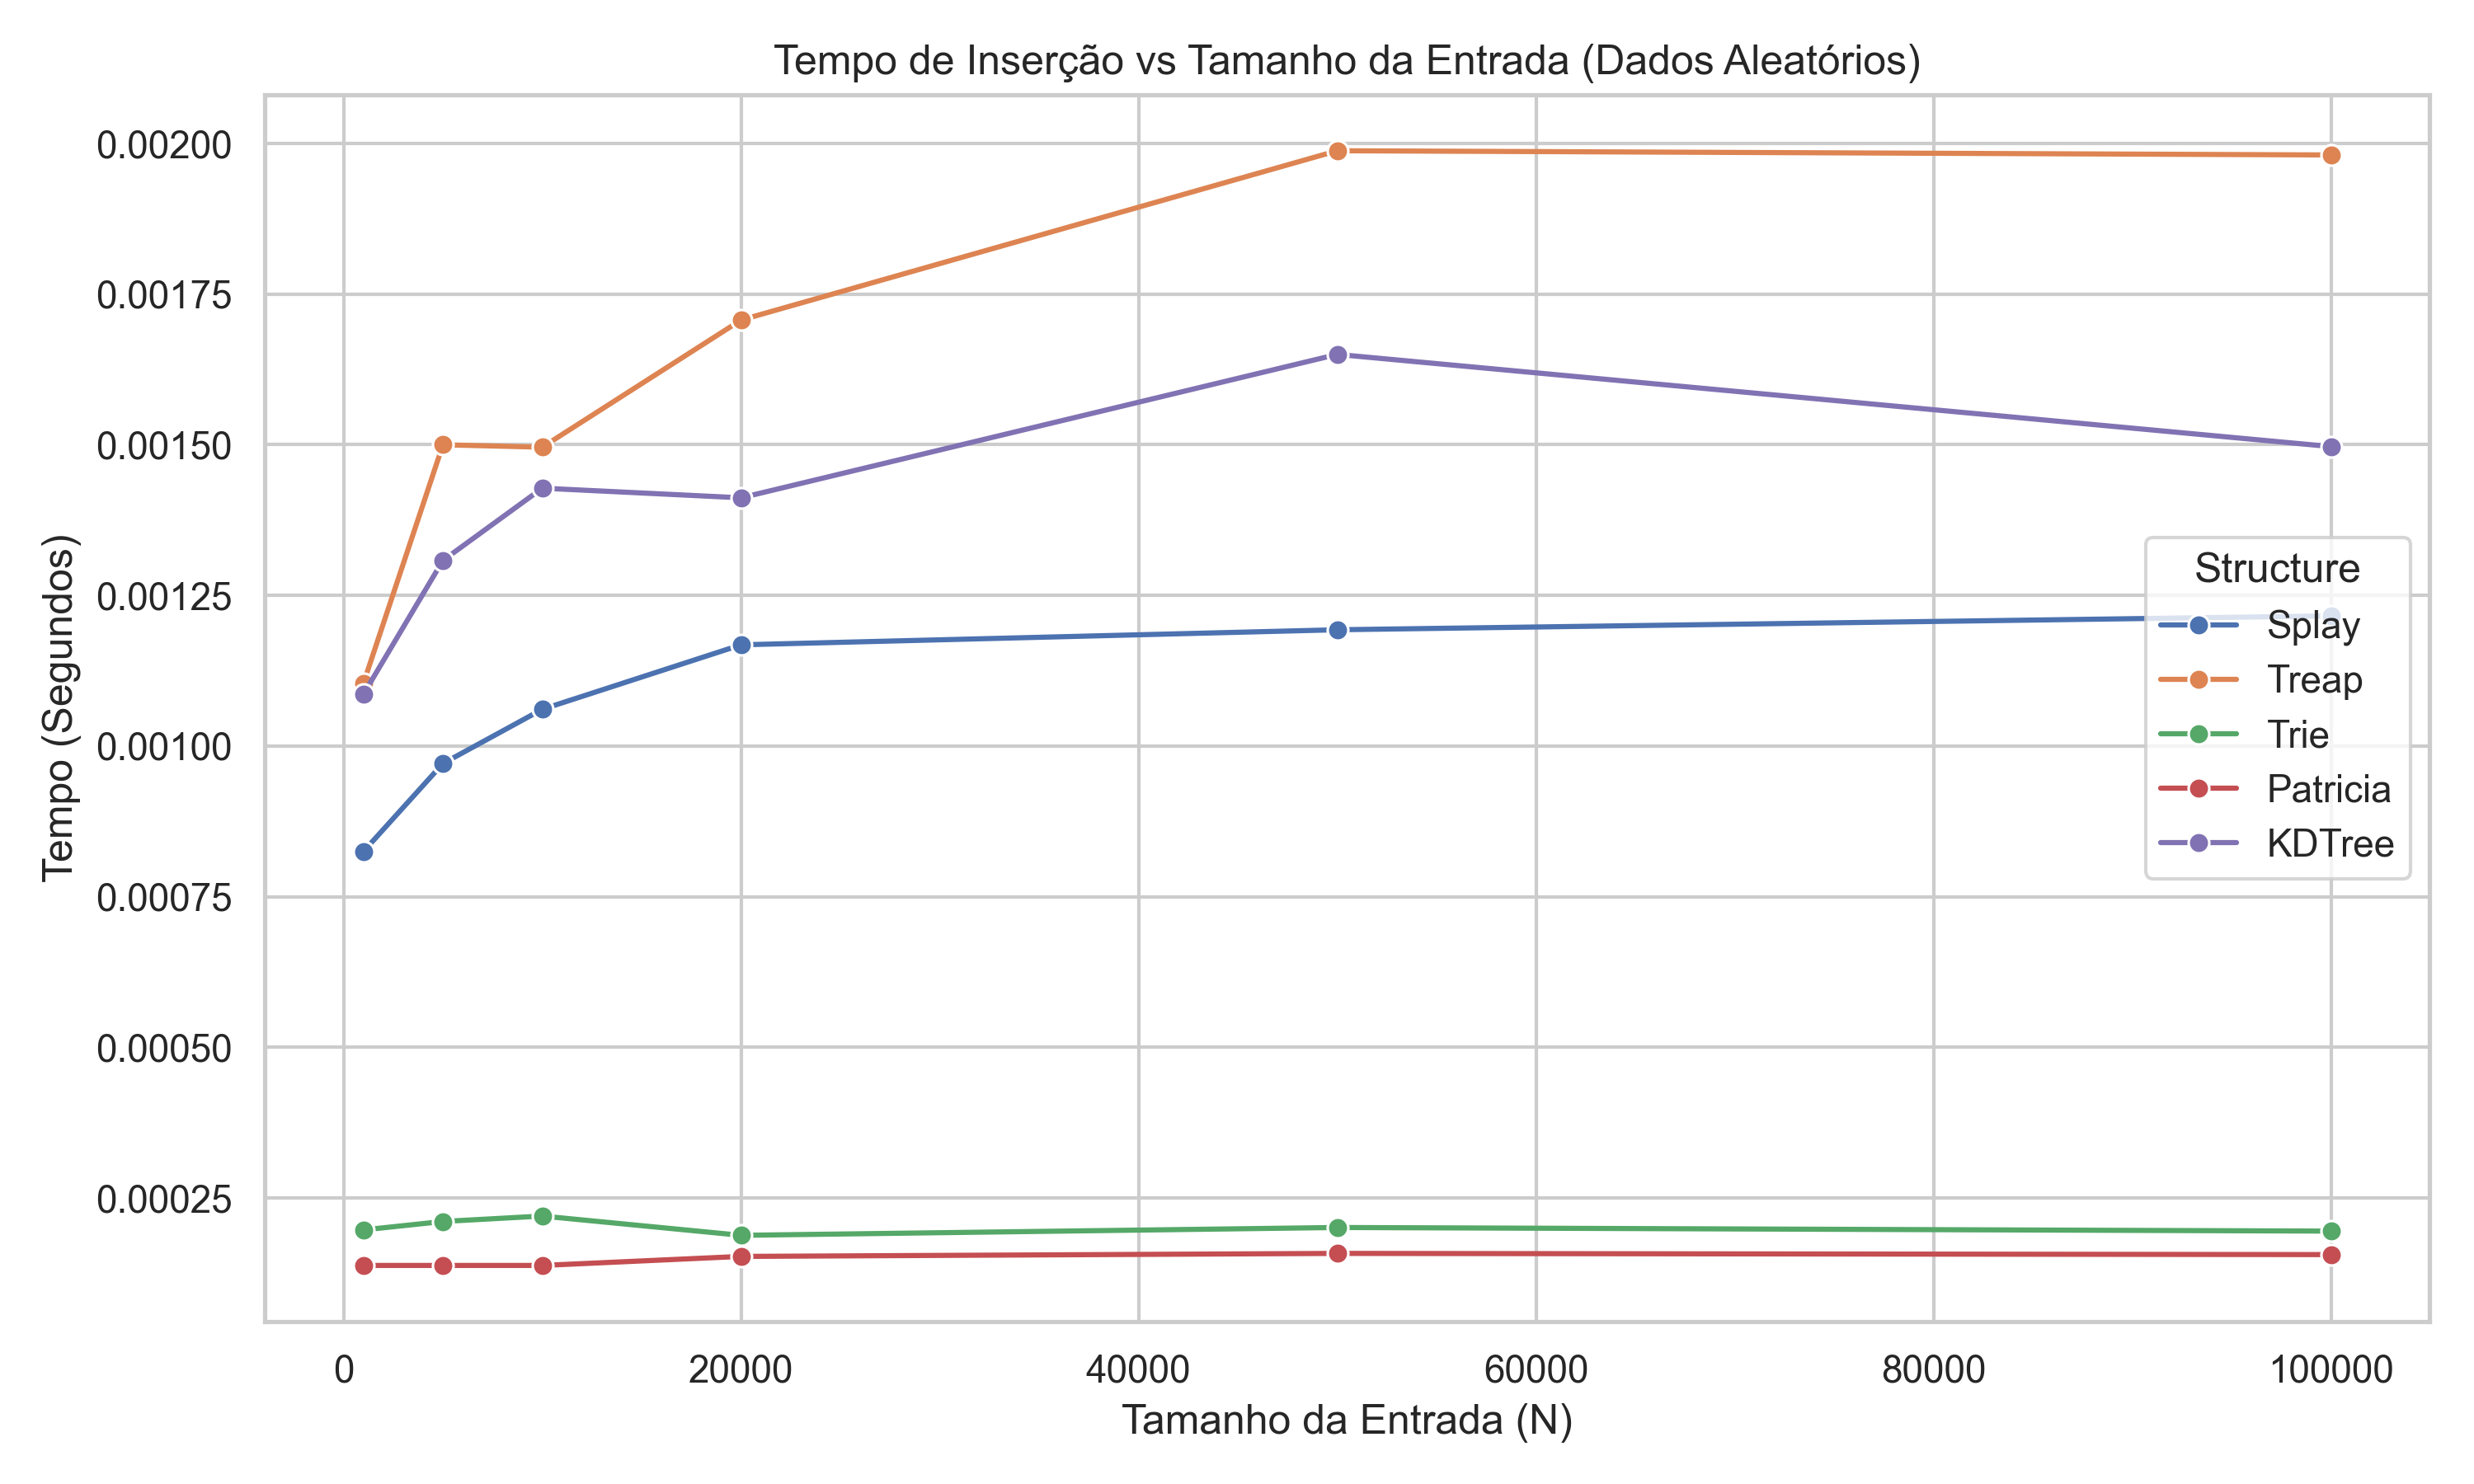
\includegraphics[width=0.75\textwidth]{insert_time_random.png}
    \caption{Gráfico de Tempo de Inserção vs Tamanho (Random Data).}
    \label{fig:insert}
\end{figure}

\subsection{Comportamento da Busca}
O tempo de busca, demonstrado na Figura \ref{fig:search}, repete o perfil assintótico da inserção, evidenciando o quão eficientes as operações \textit{Splaying} e as travessias em cadeias Trie se saem mesmo quando N assume valores próximos ao absurdo de $10^5$.

\begin{figure}[H]
    \centering
    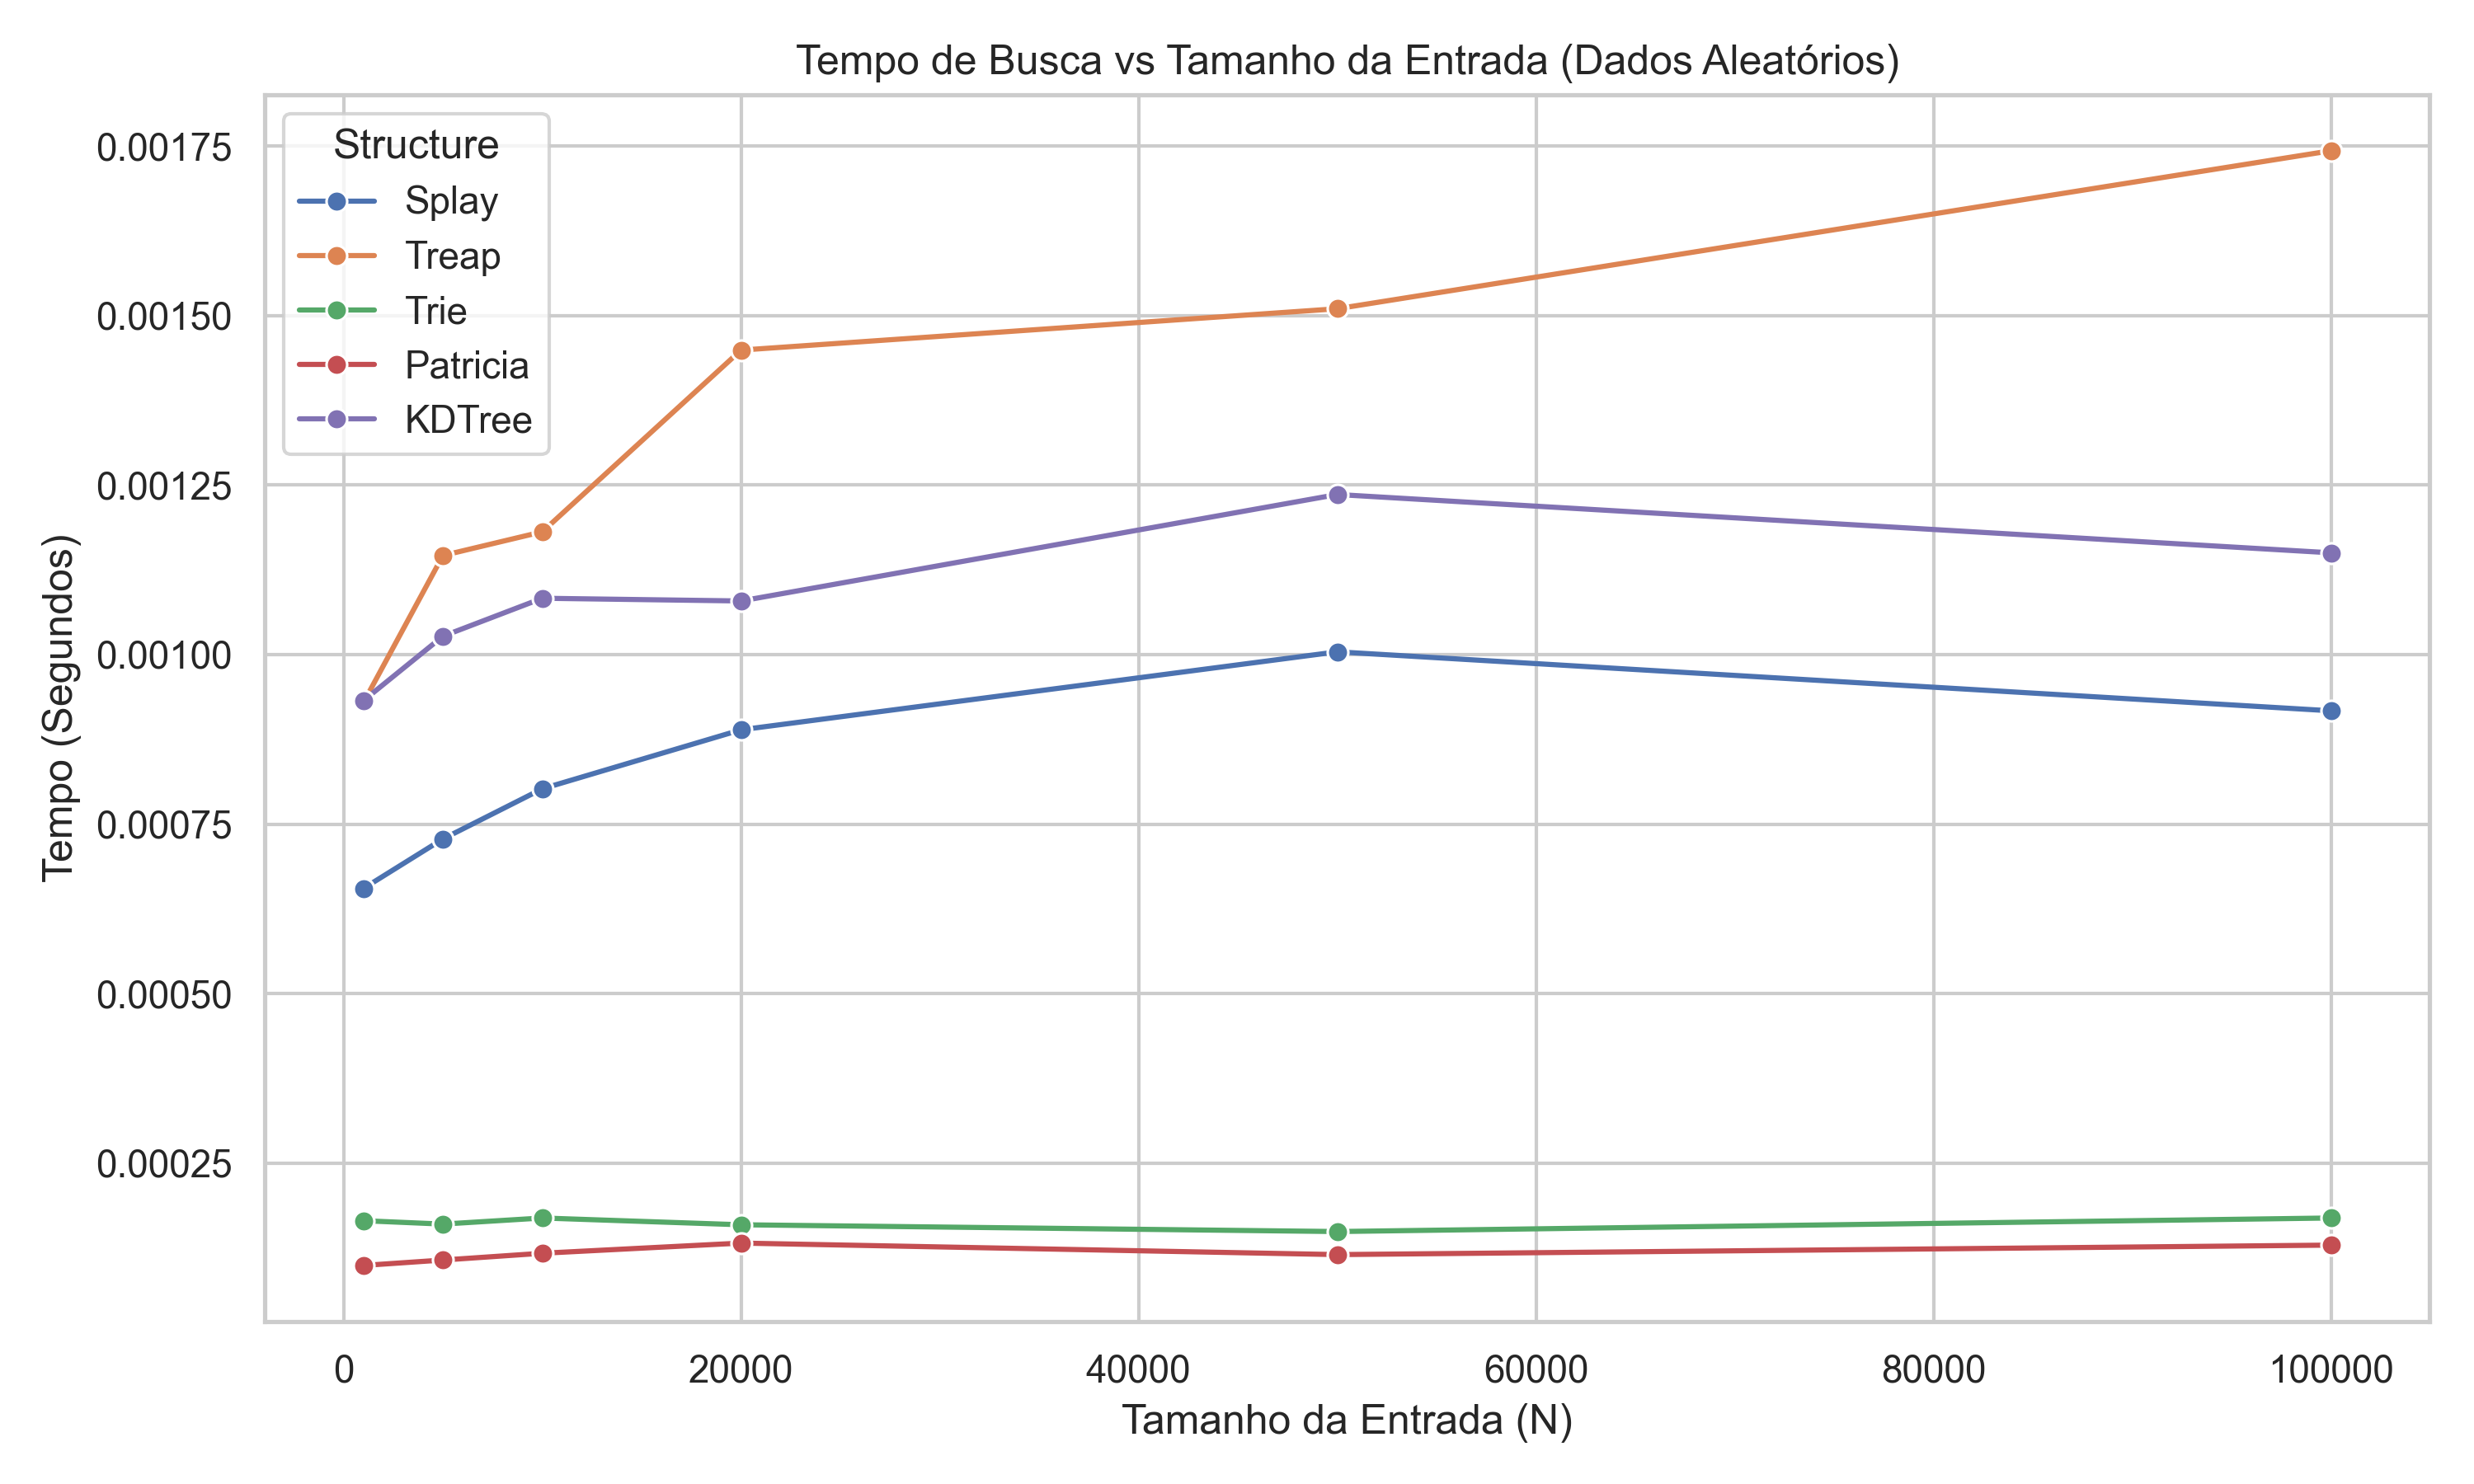
\includegraphics[width=0.75\textwidth]{search_time_random.png}
    \caption{Gráfico de Tempo de Busca vs Tamanho (Random Data).}
    \label{fig:search}
\end{figure}

\subsection{Otimização de Espaço de Memória na Patricia Tree}
Como evidenciado no referencial teórico, a Trie possui perdas cruciais de fragmentação se comparada à Radix/Patricia Tree, problema flagrante refletido na Figura \ref{fig:memory}. A compactação da Patricia a manteve com curvas de uso de memória quase tangentes às estruturas binárias tradicionais.

\begin{figure}[H]
    \centering
    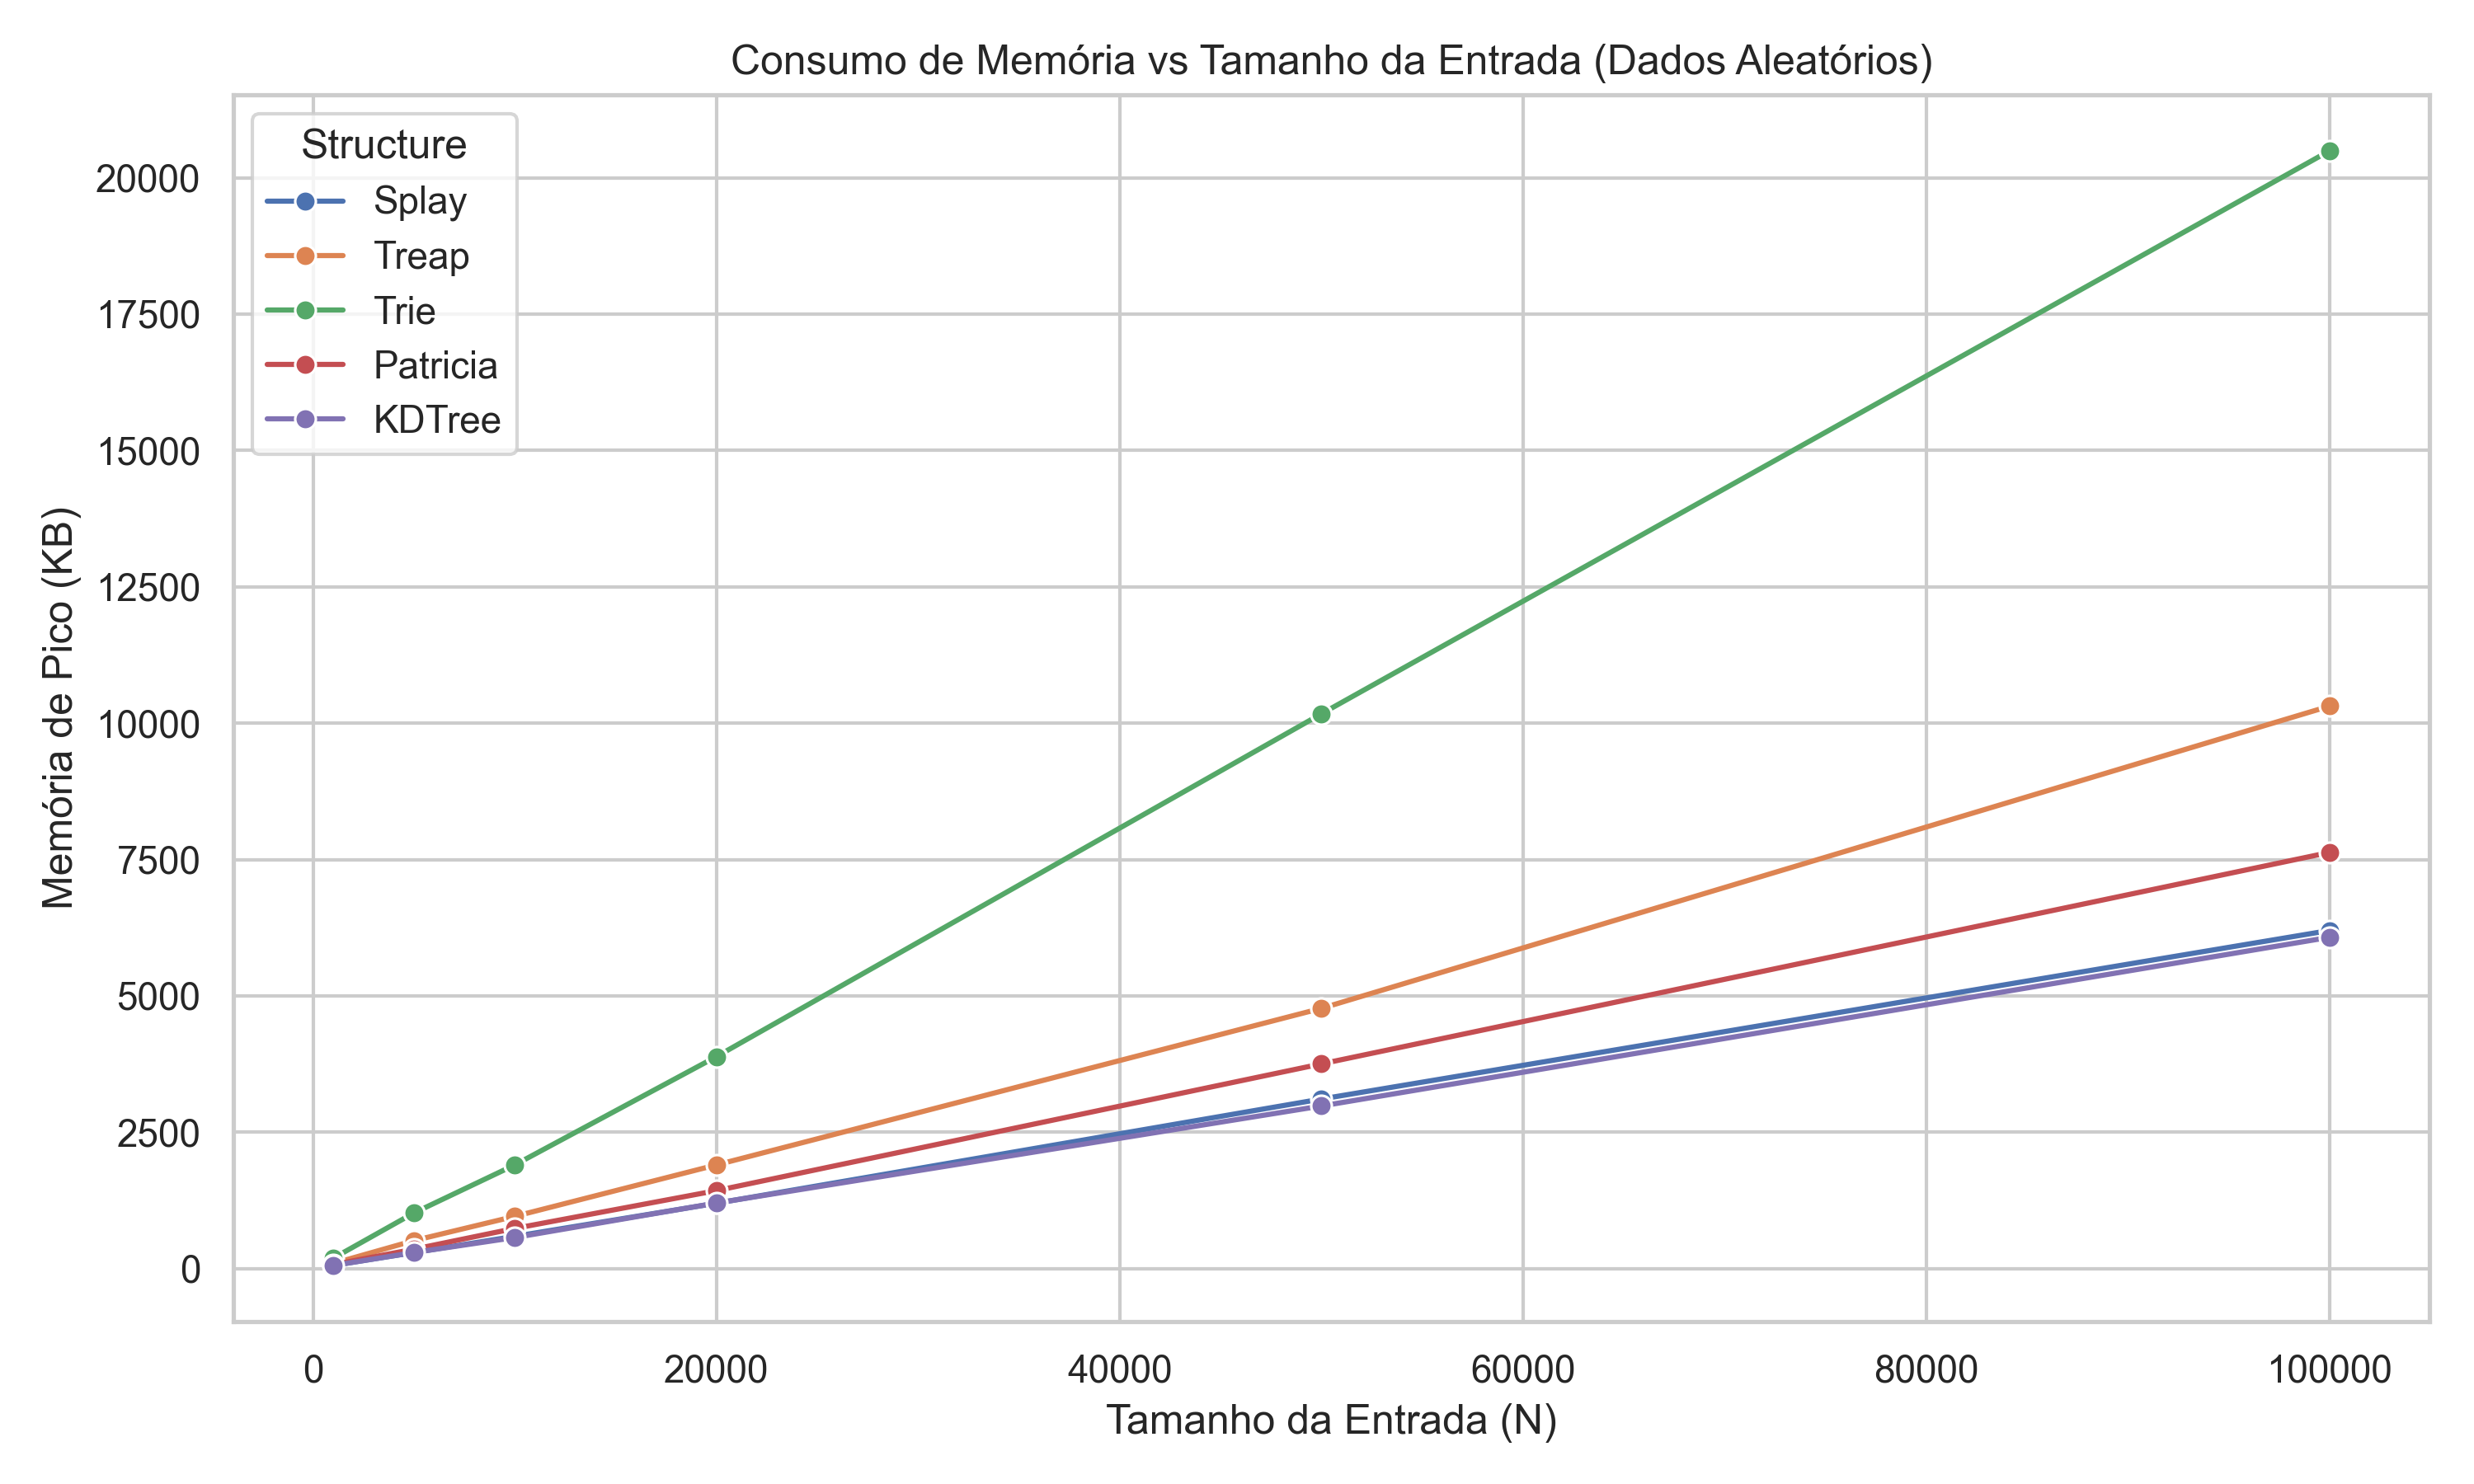
\includegraphics[width=0.75\textwidth]{memory_random.png}
    \caption{Consumo de Memória de Pico pelo interpretador vs Número de Inserções.}
    \label{fig:memory}
\end{figure}

\subsection{Sensibilidade Distribucional (Pior Caso Computacional)}
Analisando as estruturas com dados degenerados (distribuição estritamente ordenada ao longo do vetor), o gráfico na Figura \ref{fig:worst} indica as catástrofes performáticas de árvores não adaptadas, notadamente visível se a KD-Tree receber entradas como pares ordenados uniformes $(1,1), (2,2), ..., (n,n)$, reduzindo a topologia multiespacial em uma mera Lista Encadeada Linear oblíqua $\mathcal{O}(N^2)$.

\begin{figure}[H]
    \centering
    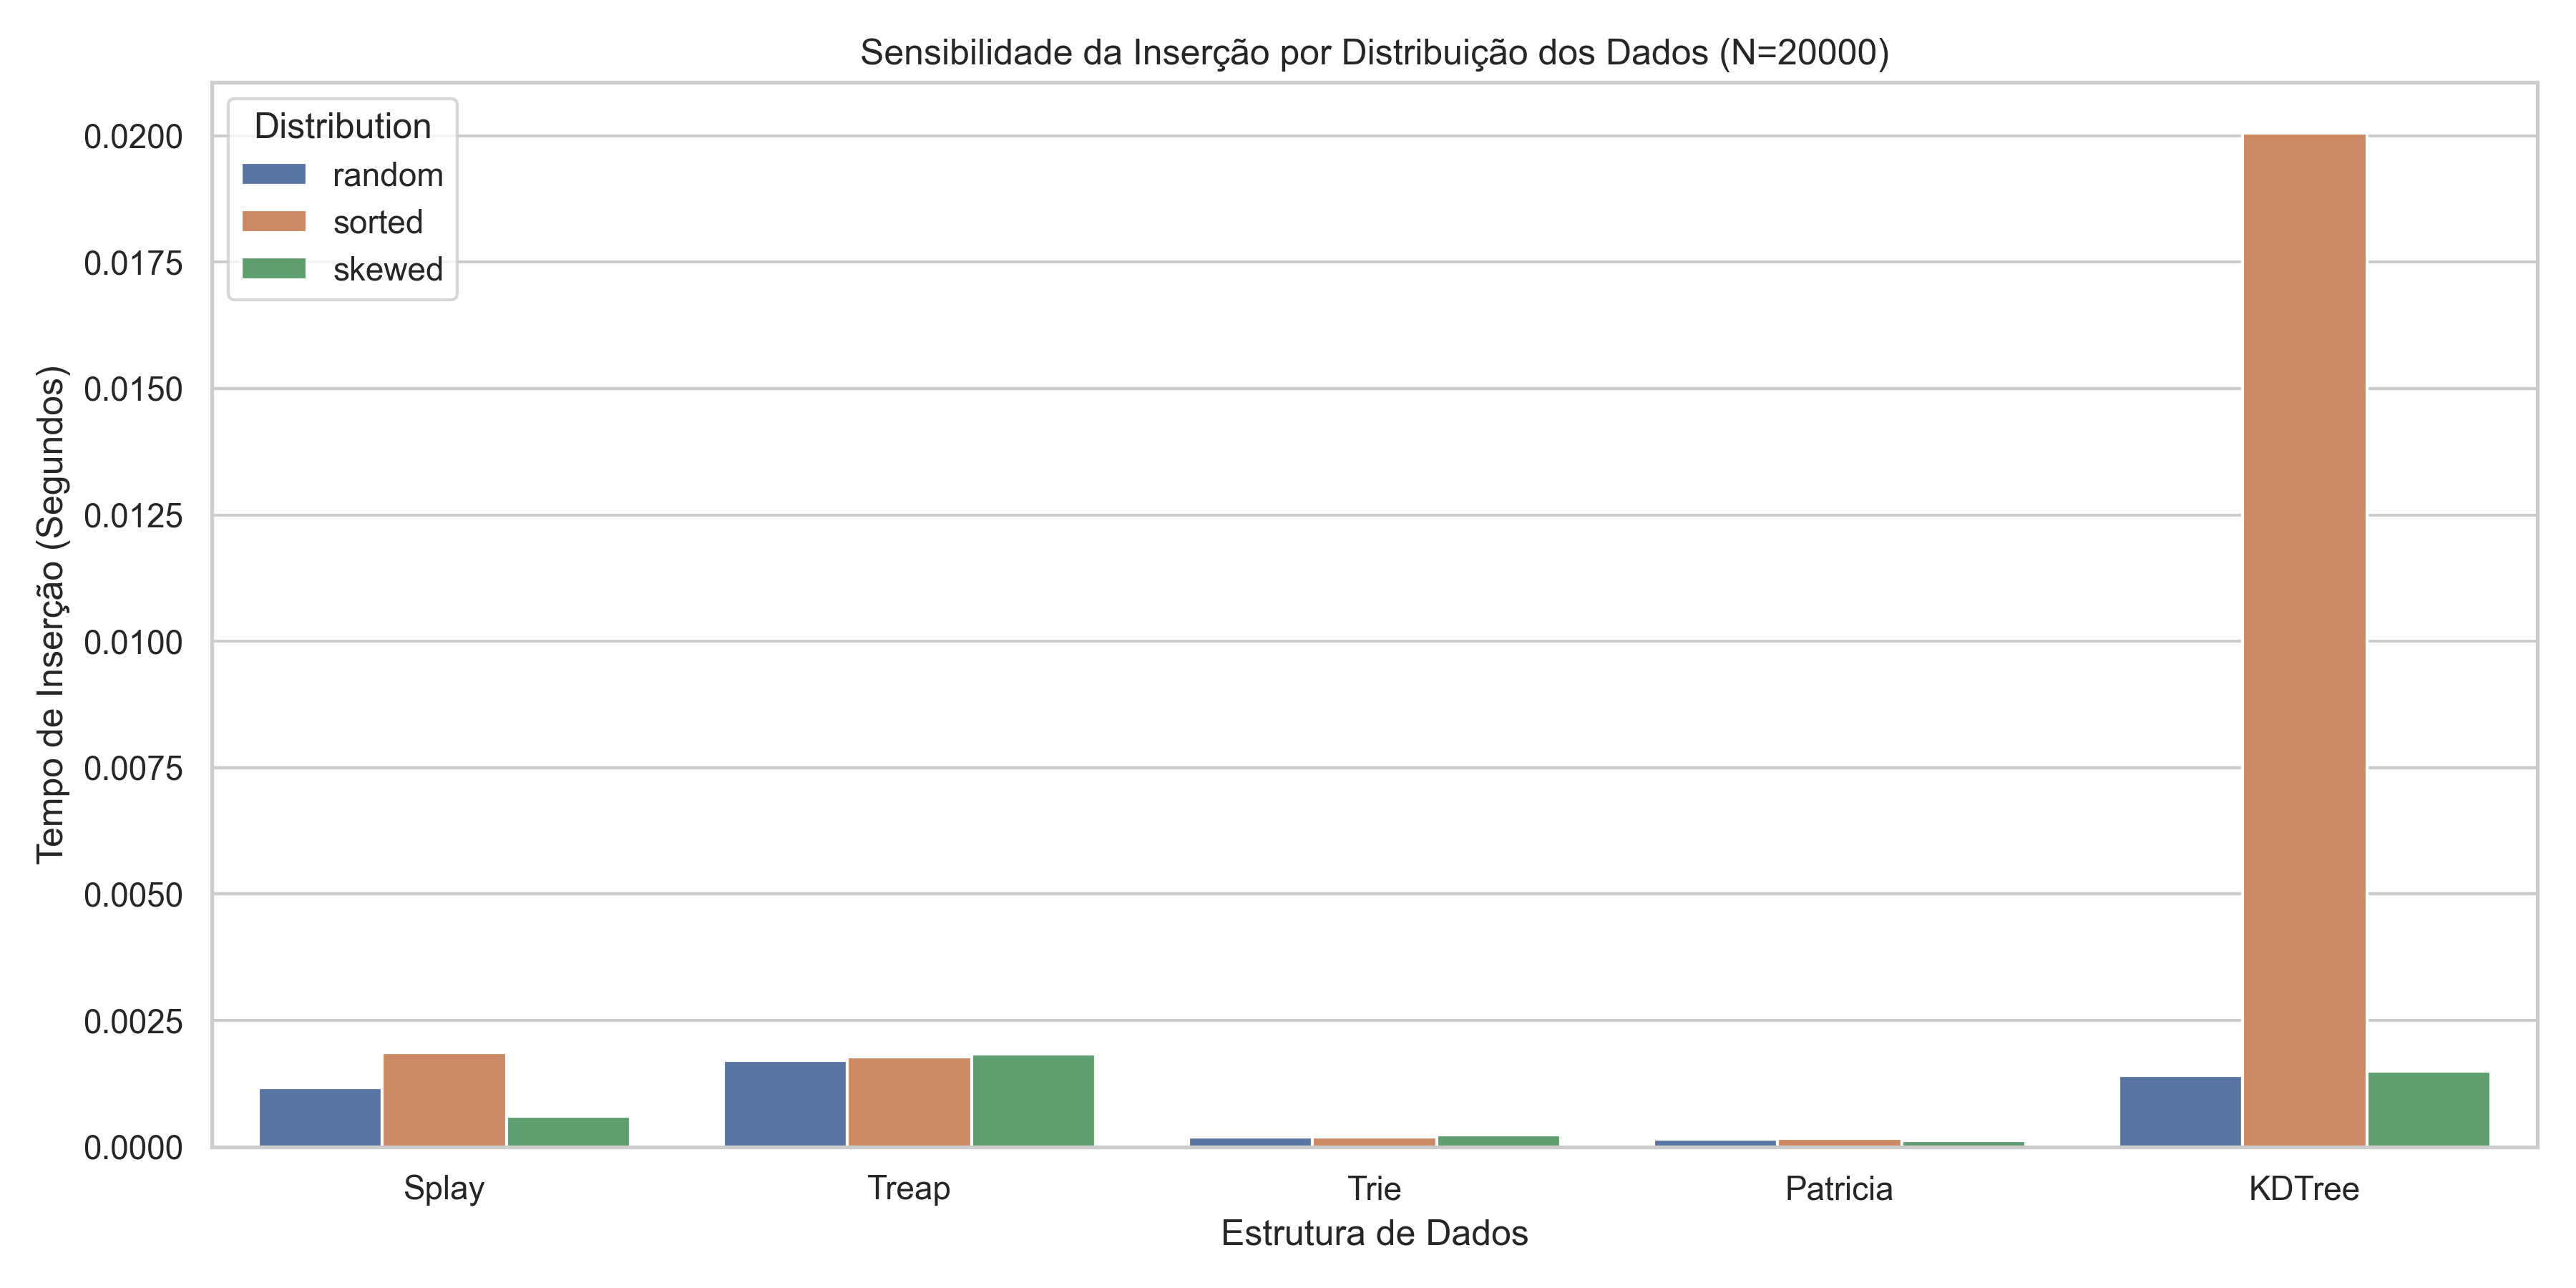
\includegraphics[width=0.75\textwidth]{distribution_impact.png}
    \caption{Impacto do pior caso computacional com N estático.}
    \label{fig:worst}
\end{figure}

\section{Conclusão}
O experimento atingiu os objetivos pretendidos na disciplina de AED 2. Verificou-se não só de modo téorico, mas visual e empírico, que as Estruturas em Árvore Avançadas são produtos engenhosos direcionados aos pormenores da arquitetura de sistemas. Enquanto a Splay Tree revoluciona o uso das premissas de localidade, a Patricia Tree mostra quão profundo o tratamento de strings pode chegar ao poupar os \textit{heaps} de RAM dos servidores modernos. Finalmente, consolidar isso em interfaces visuais modernas de smartphones prova o quão atemporais são os fundamentos da teoria da computação.

\end{document}
